\documentclass[../../main.tex]{subfiles}
\begin{document}
\graphicspath{{./figures}}
\chapter{\textit{Two-Line Element set}}\label{ap::tle}

El TLE o \textit{Two-Line Element set} es un formato de datos que codifica una lista de elementos orbitales de un objeto en órbita terrestre para un momento determinado\cite{tle-wiki}. Un ejemplo de estos parámetros y su codificación se muestra en la figura \ref{fig::valores-tle}; en la figura \ref{fig::tle} se muestra un ejemplo de el \textit{Two-Line Element set} y en las figuras \ref{fig::valores-1} y \ref{fig::valores-2} se muestra su codificación.

En el TLE se encuentra codificada toda la información necesaria para definir la órbita unívocamente. Esto permite propagar la órbita en el tiempo utilizando los parámetros orbitales.

Mas aún, para una dada localización terrestre, como una estación terrena por ejemplo, puede calcularse, empleando la información del TLE, la posición en el cielo del satélite referida a esa ubicación. Esto permitió el desarrollo de técnicas de apuntamiento basado en los TLE como se explicó en la sección \todo{poner ref}. Además, propagando la órbita de la misión de interés se puede realizar un seguimiento del satélite en el cielo desde la estación terrena, lo cual permite apuntar al satélite durante toda su pasada.

La información del TLE también fue utilizada para estimar el corrimiento Doppler asociado a un satélite respecto a la estación terrena. Esto es de gran relevancia ya que, como se explicó en \todo{poner ref}, en este proyecto resulta necesario corregir el corrimiento Doppler. Siendo este un parámetro variable dependiente de la componente radial de la velocidad relativa entre el satélite y la estación terrena, debe calcularse empleando los conocimientos de la ubicación de la estación terrena y la órbita del satélite, codificada en el TLE.

El formato TLE es un estándar de facto para la distribución de los elementos orbitales de un objeto en órbita terrestre, existiendo diversas herramientas de seguimiento de satéltites que brindan este parámetro como \textit{Orbitron}\cite{orbitron} o \textit{Gpredict}\cite{gpredict}. Estas herramientas permiten seguir y visualizar la órbita de múltiples satélites de manera simultánea, encargándose de la propagación de los TLE.


\begin{figure}[H]
    \centering
    \subcaptionbox{Ejemplo de TLE.\label{fig::tle}}
    {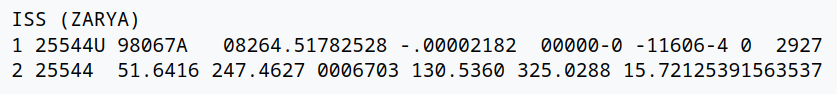
\includegraphics[width=0.9\linewidth]{tle.png}}\\[1PC]
    \subcaptionbox{Primera línea.\label{fig::valores-1}}
    {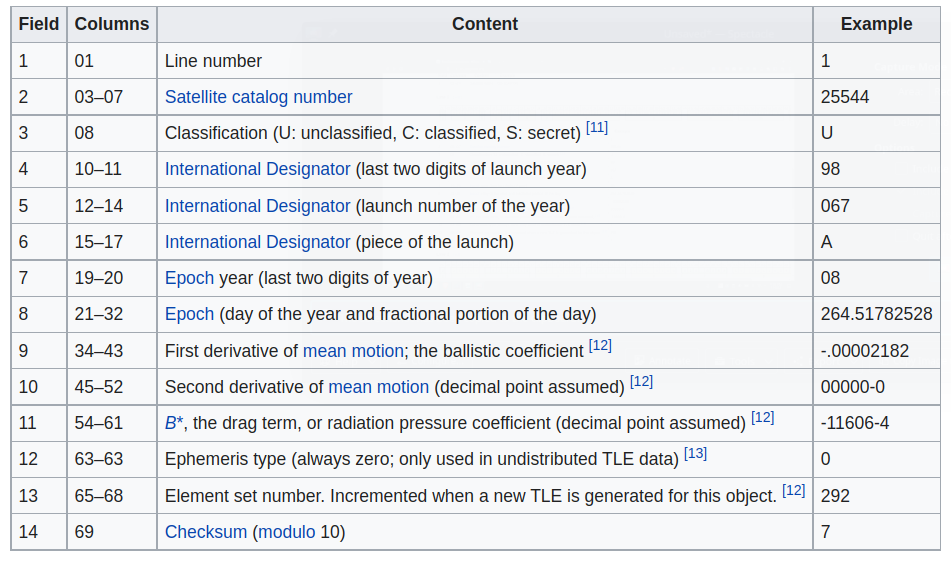
\includegraphics[width=0.9\linewidth]{valores-1.png}}\\[1PC]
    \subcaptionbox{Segunda línea.\label{fig::valores-2}}
    {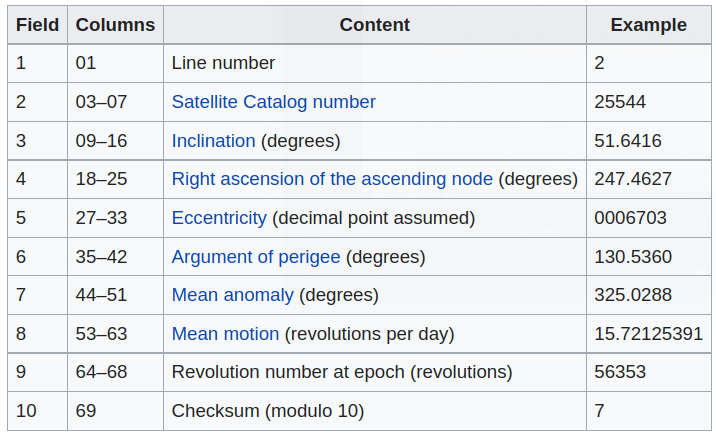
\includegraphics[width=0.7\linewidth]{valores-2.png}}
    \caption{Información codificada en las líneas del TLE junto con valores de ejemplo\cite{tle-wiki}.}
    \label{fig::valores-tle}
\end{figure}
\end{document}